
% 1. AP2 attempt of data catalog for web data https://fraunhofer-my.sharepoint.com/:x:/r/personal/nicolo_brandizzi_iais_fraunhofer_de/_layouts/15/Doc.aspx?sourcedoc=%7BBE579811-082D-4901-946A-4F864B954CB9%7D&file=FhG%20Data.xlsm&action=default&mobileredirect=true

% 2. AP3 excel for training phases 
%https://fraunhofer-my.sharepoint.com/:x:/r/personal/michael_fromm_iais_fraunhofer_de/_layouts/15/Doc.aspx?sourcedoc=%7BFFD598FC-27BE-4AC3-BF70-7FBF7BF844A0%7D&file=OpenGPT-X-7B-Training.xlsx&action=default&mobileredirect=true

% 3. AP3 link with oscar info based on focus on 4 langauges 
%https://fraunhofer-my.sharepoint.com/:x:/r/personal/michael_fromm_iais_fraunhofer_de/_layouts/15/Doc.aspx?sourcedoc=%7BF3D7F6C4-D28A-4398-9CCE-EA9C2D95050C%7D&file=OpenGPT-X%20Phase%201.xlsx&action=default&mobileredirect=true

% dump used with number of pages/docs in billion . Need to find how many tokens per page
% This data comes from here :https://fraunhofer-my.sharepoint.com/:x:/g/personal/ines_wendler_iais_fraunhofer_de/EVj7bq4zU4dKt-E6fAE6xPgBK-Z3C80nx4qAfFi9P0gjfw?e=HAxml7&wdOrigin=TEAMS-MAGLEV.p2p_ns.rwc&wdExp=TEAMS-TREATMENT&wdhostclicktime=1712751229207&web=1
% which is the billion pages per dump reported by commoncrawl cross referenced with ap3 link (#3)
% {'2014-42': 3.72, '2015-14': 1.64, '2015-48': 1.82, '2016-22': 1.46, '2016-44': 3.25, '2017-13': 3.07, '2017-47': 3.2, '2018-30': 3.25, '2018-47': 2.6, '2019-22': 2.65, '2020-24': 2.75, '2020-45': 2.71, '2021-31': 3.15, '2021-49': 2.5, '2022-27': 3.1, '2022-40': 3.15, '2022-49': 3.35, '2023-06': 3.35, '2023-14': 3.1, '2023-23': 3.1, '2017-51': 2.9, '2018-05': 3.4, '2018-09': 3.4, '2018-13': 3.2, '2018-17': 3.1, '2018-22': 2.75, '2018-26': 3.05, '2018-34': 2.65, '2018-39': 2.8, '2018-43': 3.0, '2018-51': 3.1, '2019-04': 2.85, '2019-09': 2.9, '2019-13': 2.55, '2019-18': 2.5, '2019-26': 2.6, '2019-30': 2.6, '2019-35': 2.95, '2019-39': 2.55, '2019-47': 2.55, '2019-51': 2.45, '2020-05': 3.1, '2020-10': 2.6, '2020-16': 2.85, '2020-29': 3.14, '2020-34': 2.45, '2020-40': 3.45, '2020-50': 2.64, '2021-04': 3.4, '2021-10': 2.7, '2021-17': 3.1, '2021-21': 2.6, '2021-25': 2.45, '2021-39': 2.95, '2021-43': 3.3, '2022-05': 2.95, '2022-21': 3.45, '2022-33': 2.55, '2023-40': 3.4, '2023-50': 3.35}

%60 dumps where used with the earliest being 2014-42 and the latest 2023-5 with A total of 173 billion documents 

As previously mentioned (Section \ref{sec:datasets.selection.cc}), the web data used in this project was sourced from CommonCrawl. For this study, we utilized 60 distinct dumps from CommonCrawl, spanning a broad timeframe. The earliest dump was week 42 of 2014 (2014-42), and the most recent dump was week 5 of 2023 (2023-5). This extensive range allowed us to capture a wide variety of web content across nearly a decade, ensuring that the dataset reflects both historical and contemporary web information.

On average, each CommonCrawl dump contains approximately 2.7 billion documents. Across all 60 dumps, we accumulated a total of 173 billion documents, representing around 703 terabytes of raw, unprocessed data. This vast volume of data provided a strong foundation for training large-scale language models but also introduced significant challenges in terms of data processing and filtering, as discussed in previous sections.


\begin{table}[htb!]
\centering
\begin{tabular}{cl}
\toprule
\textbf{Year} & \textbf{Week} \\ 
\midrule
2014         & 42               \\ 
2015         & 14, 48           \\ 
2016         & 22, 44           \\ 
2017         & 13, 47, 51       \\ 
2018         & 5, 9, 13, 17, 22, 26, 30, 34, 39, 43, 47, 51 \\ 
2019         & 4, 9, 13, 18, 22, 26, 30, 35, 39, 47, 51 \\ 
2020         & 5, 10, 16, 24, 29, 34, 40, 45, 50 \\ 
2021         & 4, 10, 17, 21, 25, 31, 39, 43, 49 \\ 
2022         & 5, 21, 27, 33, 40, 49 \\ 
2023         & 6, 14, 23, 40, 50 \\ 
\bottomrule
\end{tabular}
\caption{List of dumps by year and week.}
\label{tab:dumps_by_year}
\end{table}


\paragraph{Dumps}
In this section, we provide a detailed look at the CommonCrawl dumps used in our project. The dumps span multiple years, with varying distributions of weeks per year. Table \ref{tab:dumps_by_year} presents  the list of years and the corresponding weeks for each dump.

% Julich
% 2014: 42 (done)
% 2015: 14 (done), 48 (done)
% 2016: 22,(ongoing) 
% 2017: 13(ongoing), 47(done), 51(done)
% 2018: 05 , 09, 13, 17, 22, 26, 30, 34, 39, 43, 
% 2019: 51
% 2020: 05, 10,16, 29, 34, 40, 50
% 2021: 04, 31
% 2022: 27, 40, 
% 2023: 06, 14, 23, 

% Dresden
% 2014:
% 2015:
% 2016:
% (2018): 47, 51
% 2019: 04, 09, 13, 18, 22, 26, 30 , 35, 39,  47
% (2020): 24, 45
% (2021): 10, 17, 21, 25, 39, 43, 49
% (2022): 05, 21, 33, 49, 
% 2023: 40, 50

% Missing
% 2014:
% 2015:
% 2016: 44
% 2018: 
% 2019: 51
% 2020:
% 2021: 
% 2022: 
% 2023:



As can be seen from the list, the distribution of dumps across weeks is uneven. Earlier years, particularly 2014 through 2016, have fewer weeks represented compared to more recent years. However, the dumps from these earlier years typically contain a higher dump density, i.e. average document size (see Figure \ref{fig:dumps_distribution}). After 2017, CommonCrawl transitioned to a strategy of producing more frequent dumps, each with relatively smaller average document sizes.

This shift in strategy has important implications for data processing. Special attention must be paid to the earlier years (2014–2016), where deduplication can be more computationally expensive due to the larger document sizes. In these cases, employing stricter filtering mechanisms may be necessary to ensure efficient processing and to avoid excessive resource consumption during deduplication.


% DATA for graphs
% years 2014 2015 2016 2017 2018 2019 2020 2021 2022 2023
% len(year) 1 2 2 3 12 11 9 9 6 5
% size(year) 22.53 17.98 16.91 37.28 36.3 32.15 25.69 26.15 18.55 16.3
% avg(size(year)) 22.53 8.99 8.455 12.426 2.025 2.922 2.854 2.905 3.091 3.260





\begin{figure}
\centering
  \centering
  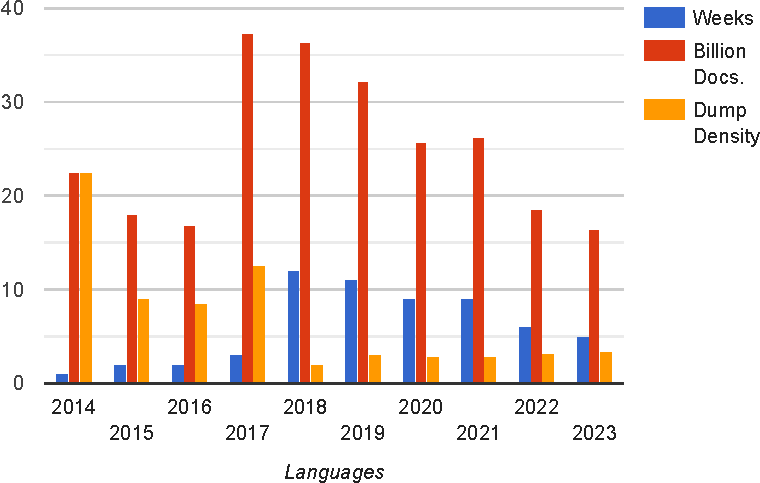
\includegraphics[width=0.75\linewidth]{images/Analysis/docs_weeks_density_xyear.pdf}
\caption{Analysis of CommonCrawl dumps used in the dataset, showing the distribution of dump weeks (blue), billion documents (red) and average dump density (yellow) per year.}
\label{fig:dumps_distribution}
\end{figure}



\paragraph{Compute power}

% For these numbers i used benny's 'dedup_cpu_requirements.html'. Specifically, step 2, old estimate. I tool the total for en 210, computed the percentage going in dedup and filtering. Used that percentage on the total estimated BEFORE code (504k), divided by 110 to get the "per dump" and then tiems 60 to get the total 
Tracking the compute power required during data processing is essential for planning and securing the necessary resources. A well-structured plan not only ensures that adequate resources are available but also provides an opportunity to analyze computational efficiency and sustainability.

Below, we estimated total CPU hours consumed at each stage of the pipeline:

% \todo[inline]{BS: I don't know how you got those numbers? (Perhaps it would also be interesting for the reader - if it is not too complicated to explain\dots NB: fill out footnote) }

\begin{itemize}
    \item Conversion: On average, converting a dump takes 115,2 CPU hours. For all the data combined this stage took 6,912 CPU hours.
    \item Filtering: On average, filtering one dump takes 763 CPU hours. For all dumps combined, this stage required 45,810 CPU hours. 
    \item Deduplication: Deduplication is notably resource-intensive, taking an average of 3,680 CPU hours per dump. For the entire dataset, this stage consumed 221,230 CPU hours. 
\end{itemize}


Deduplication is by far the most time-consuming step, consuming 80.8\% of the total compute power, which is why it is kept as the final stage in our pipeline (see Section \ref{sec:pipelines.web.dedup}). This is followed by filtering, which takes 16.7\%, and conversion, accounting for 2.5\%.


% \paragraph{Filtering effect}
% \todo{NB: todo}


\paragraph{Deduplication Effect}

\begin{figure}
  \centering
  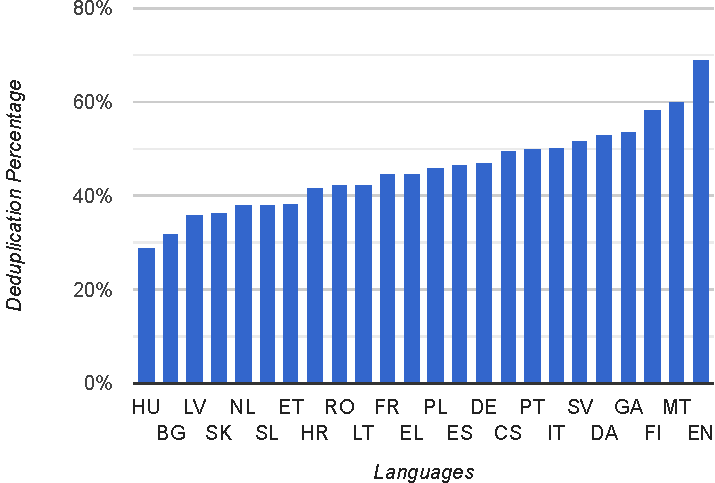
\includegraphics[width=0.7\linewidth]{images/Analysis/dedup_perc_lang.pdf}
  \caption{ Percentage of data removed after deduplication for each language, showcasing the varying impact of deduplication.} 
  \label{fig:dedup_perc_lang}
\end{figure}


% Data from link #2 showing percentage of dedup data for each language taken from tab 'phase 1'
%HU BG LV SK NL SL ET HR RO LT FR EL PL ES DE CS PT IT SV DA GA FI MT EN
% 0.2903 0.31920000000000004 0.35969999999999996 0.3635 0.38 0.3812 0.3825 0.4164 0.4218 0.4235 0.4458 0.44630000000000003 0.46049999999999996 0.4656 0.46840000000000004 0.4953 0.4996 0.5047 0.5156000000000001 0.5301 0.537 0.5827 0.5993999999999999 0.6895

Our deduplication methodology is based on a MinHash + Locality Sensitive Hashing approach that is explained in detail in \cite{leveling_helmer_etal2024}, where the choice of algorithm, along with precision and recall metrics, are analyzed. 
In this section, we shift focus to examining how deduplication disproportionately affects different languages. Figure \ref{fig:dedup_perc_lang} illustrates the percentage of data removed after deduplication for each language, ranging from a minimum of 29.03\% for Hungarian to a maximum of 68.95\% for English. While it may seem intuitive to correlate the deduplication percentage with data availability, a Pearson correlation analysis reveals only a modest positive correlation of 0.54 (p = 0.006).

This suggests that some languages may be subject to an ``unfair'' amount of deduplication relative to their size. Although deduplication operates by identifying and removing similar content, this implies that certain languages contain a higher proportion of similar data, which may result in a final model that struggles to capture linguistic nuances.


To evaluate this disproportionality, we introduce the \textit{Deduplication Disparity Index} (DDI), which measures the impact of deduplication on each language relative to its available web data. For each language \( l \), the DDI is calculated as the Z-score of the deduplication-to-data ratio \( R_l \), which measures the percentage of data deduplicated in relation to the total web data available for that language:


\[
\operatorname{DDI}_l = \frac{R_l - \mu_R}{\sigma_R}, \quad \text{where} \quad R_l = \frac{d_l}{W_l}
\]



Here, \( d_l \) is the deduplication percentage for language \( l \), \( W_l \) is the total number of web data words for language \( l \), \( \mu_R \) is the average deduplication-to-data ratio across all languages, and \( \sigma_R \) is the standard deviation of the deduplication-to-data ratios. This Z-score transformation centers the $\operatorname{DDI}$ around zero, highlighting languages where deduplication has a disproportionately high or low impact.

Languages with a high positive Z-score, such as Maltese ($\operatorname{DDI}_{mt}=4.519$) and Croatian ($\operatorname{DDI}_{mt}=1.0735$), are significantly impacted by deduplication, while others have scores closer to zero ($\operatorname{DDI} = -0.25 \pm 0.012)$, indicating a more balanced deduplication-to-data ratio. This metric provides a systematic way to assess fairness in the data processing pipeline and highlights languages that might require further attention during preprocessing.

% \todo[inline]{BS: Are the DDIs shown somewhere in a table or diagram? NB: no, i think we have enough tables already, maybe in revised }

\subsubsection{Summary} 
The web data for this project was sourced from 60 distinct CommonCrawl dumps spanning 2014 2023, resulting in a total of 173 billion documents (703 terabytes of raw data). This broad timeframe captures both historical and contemporary web content.

Deduplication was the most resource-intensive step, consuming 80.8\% of total CPU hours allocated for data processing. We introduced the Deduplication Disparity Index (DDI) to identify languages disproportionately affected by deduplication, highlighting the need for tailored processing strategies to ensure fairness and data quality. 

